
% SGX survey dump for now... shoudl edit if time permits

% \section{Introduction}

% 	Virtualization allows multiple guests to run on a hypervisor in isolation. In 2007 researchers at InvisibleThings Labs\cite{Rutkowska_Tereshkin_2007} demonstrated that a malicious guest VM could subvert the host through the hypervisor and subsequently gain priviliged access to other guests. Variants were released for Xen, kvm, and VMWare to demonstrate applicability to both type1(bare metal) and type 2(ontop host OS) hypervisors. Amazon Web Services is the largest Cloud Service Provider (CSP) and manages over 1 million clients. Its commercial cloud services run on a modified Xen hypervisor. 
	
% 	Given the cost savings in infrastructure management and the scalability that CSPs offer, businesses are increasingly migrating their enterprise applications onto the cloud. The isolation that hypervisors alone offer isn't enough to guarantee protection of sensitive business intellectual property. Virtualization abstracts resource management issues away from development operations, but under the hood applications from different, possibly competing customers access the same memory and processors in hardware. The applications running on the cloud have the potential to be accessed or modified by neighboring guests on the same hypervisor, support staff with access to at the hypervisor level, or even malicious actors along the supply chain of the components that comprise the cloud infrastructure. 
	
	In 2007 researchers at InvisibleThings Labs\cite{Rutkowska_Tereshkin_2007} demonstrated that a malicious guest VM could subvert the hypervisor through the host and subsequently gain privileged access to other guest VMs. Intel has since developed a solution to prevent unauthorized access or modification to an application even if an attacker owns the underlying hypervisor. This section will explore the SGX architecture components and their interactions, and review attacks against the current SGX implementation. 
	
\begin{figure}
\centering
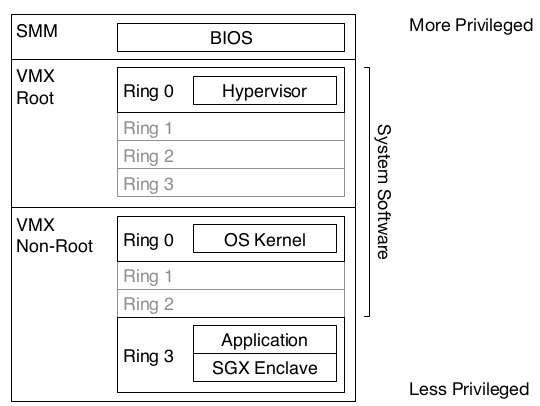
\includegraphics[scale=.4]{img/sgx/privs.png}
\caption{Virtualization Privilege Levels \cite{Shriraman_Dwarkadas_2010}}
\end{figure}

% \section{SGX Overview}
SGX (Software Guard Extensions) is Intel's latest evolution of trusted computing hardware following TPMs (Trusted Platform Module) and TXT (Trusted eXecution Technology). It allows trusted software to run on remote inherently untrusted systems while ensuring:

\textbf{Integrity} - by preventing the remote system from altering the program execution environment

\textbf{Confidentiality} - by only decrypting data inside the CPU to prevent even higher privileged processes from accessing decrypted data.

The SGX security functionality uses secure enclaves to isolate sensitive data and code from everything else in the deployed environment.In the next sections this paper will review the individual components of SGX, describe how these pieces work together to attempt to provide trusted computing on untrusted platforms, and finally examine some weaknesses in SGX that have been exploited to circumvent the desired protections.


\subsection{SGX Components}


SGX is a set of hardware, firmware, and extensions to the x86 instruction set that allow a user to create secure enclaves. A secure enclave is a hardware protected memory address space that allows execution of a trusted program on an untrusted platform with guarantees on the integrity and confidentiality of the program resources. This prevents processes running at higher privilege levels than the program itself from viewing or modifying the program's data and code. These malicious privileged processes could be executing from the operating system, hypervisor, BIOS or firmware, or even compromised microcode in the system's processor. A side effect of this protection is that debugging a running enclave is prohibited. 

SGX details below are summarized from the seminal work by Costan and Devadas \cite{Costan_Devadas_2016} unless otherwise noted, with images borrowed from the related papers \cite{Sony_DRM, SGXinpractice,Xu_Cui_Peinado_2015,Shriraman_Dwarkadas_2010, Schwarz_Weiser_Gruss_Maurice_Mangard_2017, Rutkowska_Tereshkin_2007, Rozas_2013, Costan_Devadas_2016, Brickell_Li_2009}

\textbf{Hardware Secret Keys} - As part of the manufacturing process, each SGX chip is issued two 128 bit secret keys from Intel's key generation facility. These keys are burned into e-fuses that are included on the chip's die. The two keys are the Provisioning Secret which is used in the generation of the SGX root derivation key, and the Sealing Secret, which is used in the enclave sealing and attestation processes described later. 

\textbf{Enclave Memory Encryption} - SGX uses internal CPU caches to hold decrypted data. The architecture acts as a gatekeeper by enforcing access control logic that only allows the guarded application access to decrypted data. During context switches or paging the CPU cache is encrypted again before being written out to unprotected memory.

\begin{figure}[H]
\centering
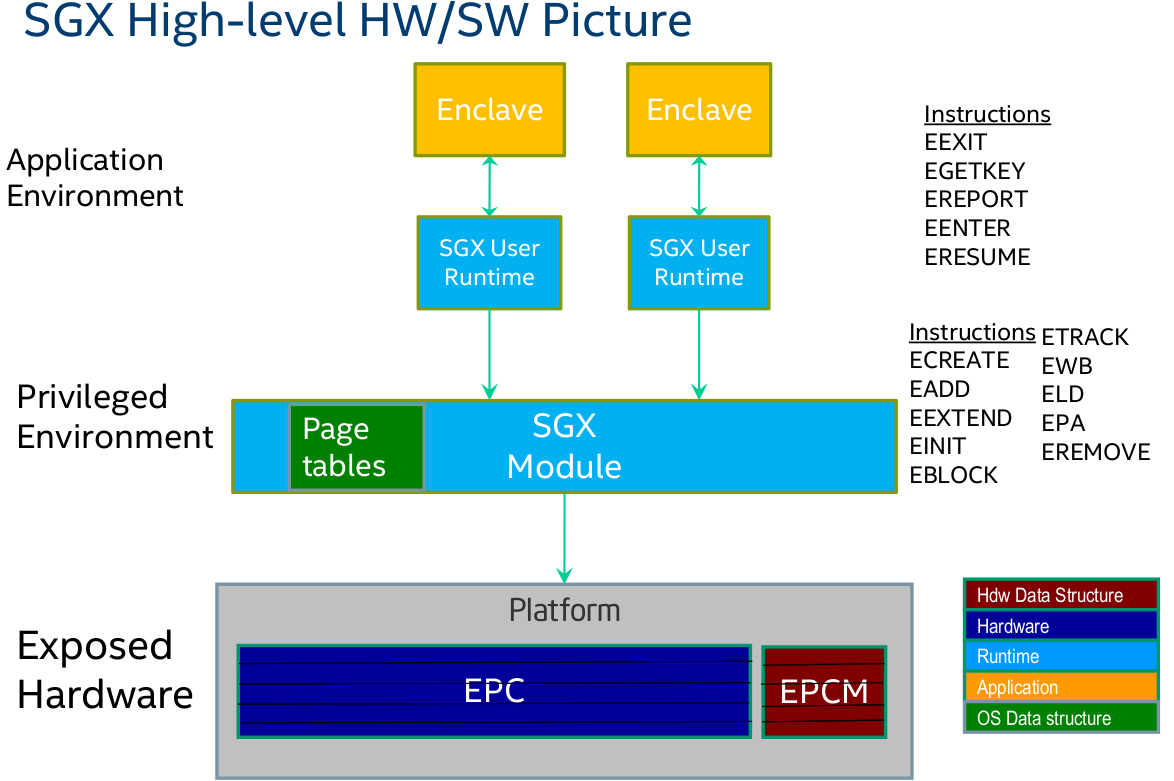
\includegraphics[scale=.2]{img/sgx/arch2.png}
\caption{Images recovered from \cite{Xu_Cui_Peinado_2015}}
\end{figure}


\textbf{Remote Attestation} - This is the crux of SGX. Remote attestation gives remote users a proof that an enclave is running a given
program securely. You can see it as a public key certificate where a trusted entity endorses a program (the enclave) rather than a
public key.

\textbf{Sealed Storage} - To keep secrets provisioned by a remote user, SGX-enabled CPUs can store these secrets as encrypted BLOBs
outside the CPU, protecting their confidentiality and integrity.

\textbf{EPC} - Envlave Page Cache - (bottom of diagram) in hardware. Memory access semantic does extra checks beyond what was done before in non-SGX systems, where accesses went through the page table to find address translation and then went to memory to read in contents. EPC does additional checks to make sure the access request originates from a process inside the enclave and checks that the linear address the enclave was built for is the same as that requested to protect from the OS trying to remap pages. The EPC also checks if the application wants this area to be read/write capable. 

\textbf{EPCM} - Non enclave software is not permitted to access the EPC as governed by the enclave access control logic. In order to perform access checks on a memory read request, the Enclave Page Cache Map (EPCM) maintains an array in SGX protected memory containing an element for each EPC page. This element tracks the owner of the page  [\textbf{ENCLAVESECS}], the page type [\textbf{PT}], and whether or not the page is valid [\textbf{VALID}]. The VALID bit prevents EPC instructions from operating on pages that are already in use. The page type PT is marked 'regular' for enclave code and data pages. SGX support structure storage pages are marked according to type, for instance PT\_SECS delineates SGX Enclave Control Structures. Controlled entry points into the enclave memory space prevent also return-oriented programming (ROP) attacks. Use EEnter instruction to gain access to memory space, all other accesses are prevented by SGX hardware.

\textbf{ECREATE} instruction used to setup/instantiate the enclave. Then use EADD to add data and code to the page cache one page at a time. 

No secrets used or crypto used to setup the enclave. Once code or data to be protected is loaded the enclave is sealed to protect from unauthorized access. Measurements are taken from cryptographic hashes of the built environment. These measurements are secured and reproduced on the deployed system to verify the integrity of the enclave. 

\textbf{EINIT} - declare the enclave is fully built. The enclave can now be entered. 

\textbf{EBLOCK ETRAC EWRITEBACK ELOAD} - paging instructions to facilitate loading pages into main memory and back to disk while maintaining security properties listed above. 

\textbf{EPA} - versioning for paging. 

\textbf{EREMOVE} - take out pages for an inactive enclave. 

\textbf{EGETKEY} - security instructions used to seal data based on enclave measurement (enclave key) 

\textbf{EREPORT} - hardware instruction used to verify enclave is running shielded on a valid Intel SGX system. 

\textbf{MRENCLAVE} - measurement enclave. keeps running hash of the enclave. This is similar to TPM to keep running hash. 

\begin{figure}[H]
\centering
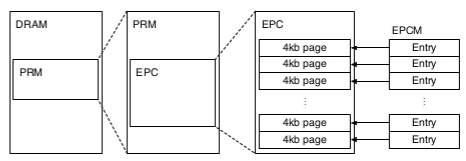
\includegraphics[scale=.4]{img/sgx/epc.png}
\caption{Enclave Page Cache \cite{Costan_Devadas_2016}}
\end{figure}

\textbf{Enclave Setup Flow:}

\textbf{1.} Starting with virtual address space and physical address space. ECREATE declares a memory range in virtual address space that will be used for the enclave. The enclave page cache (EPC) defined at system start time and EPCM both removed from system memory map to be used for SGX operations. 

\textbf{2.} MRENCLAVE keeps running hash of the enclave (described below) using EEXTEND on each page loaded into enclave memory. Plaintext code/data is moved into shielded EPC using the EADD instruction and EPCM is updated to show linear(virtual) address of the page flagged as valid with enclave ID. Continue this until the enclave code/data is loaded. 

\textbf{3.} Once the enclave is loaded it is declared executable using EINIT. Enter and exit the enclave using EENTER and EEXIT. 

\textbf{4.} EREMOVE when enclave is no longer needed to null out enclave memory and EPCM and return to system memory map.


\begin{table}
\centering
  \caption{Useful SGX Commands}
  \label{tab:cmds}
  \begin{tabular}{ccl}
    \toprule
    Instruction & Description\\
    \midrule
    \texttt{ECREATE} & instantiate the enclave  \\
    \texttt{EINIT}& declare the enclave is ready\\
    \texttt{EBLOCK ELOAD }&  facilitate loading pages\\
    \texttt{EREMOVE }& take out inactive page \\
    \texttt{EGETKEY}& used to seal enclave\\
    \texttt{EREPORT}&  verify enclave\\
    \bottomrule
  \end{tabular}
\end{table}
% end the environment with {table*}, NOTE not {table}!

\textbf{Enclave Access Control}: There are 2 areas of access control. 
* On processor access control prevents decrypted memory region accesses from any process not within the shielded enclave. This is accomplished by the hardware checking every page table request to identify if it is mapped into the currently running enclave address space. If the request is for data within the currently loaded enclave, the processor first verifies the system is in enclave mode, then validates the request originated from within the enclave belonging to the memory being requested. If any checks fail a page fault is signaled. \cite{Schwarz_Weiser_Gruss_Maurice_Mangard_2017}

* Off chip - uses encryption to protect any code/data not currently being used in the decrypted CPU cache. Any time data/code is paged out the hardware encrypts the page with AES-128 using the root provisioning key before it is placed in the commonly addressable memory space. Encrypted pages are still under protection of the chip's access control system to prevent encrypted memory access or overwrite. 

Once the enclave has been initialized, proving the shielded application is running under SGX protection is the domain of attestation and sealing. 	

\textbf{Attestation} - When building an enclave, SGX maintains a cryptographic log of all code, data, stack and heap states, along with page locations and security flags of the trusted computing base. A 256 bit digest of this log is maintained in the MRENCLAVE. 

To verify the TCB, the verifier needs to compare the measurements of the enclave's TCB and the expected TCB. This is known as attestation. Attestation can occur locally between enclaves on the same platform, or remotely between enclaves on different platforms. 

Local attestation uses the EREPORT instruction to bind the target MRENCLAVE's report hash to the requestor's report key using symmetric cryptography. Remote attestation uses an attestation server as a middle man to verify using a global identifier called EPID (enhanced privacy identification). The quoting enclave and the enclave to be verified both use asymmetric cryptography based on the EPID(iso standard) to communicate with the attestation server in an anonymous protocol. This is the same mechanism used in TPM remote attestation. 



\subsection{Cryptography in SGX}

\textbf{Trusted Computing Base} (TCB): The boundary of what will be guaranteed secure and protected. For SGX this includes th CPU's package boundary including integrated circuits, registers, and the cache, as well as software components defined by the developer. Syscalls and interrupts are not permitted within the enclave TCB to prevent leaking and exploitation. When developing an enclave guarded application, Intel assumes the entire development machine is trusted and free from malware. 

In general, paging allows the operating system to over commit the available memory by evicting the least used memory pages to a slower storage area. EPC pages are prevented from being evicted by the OS due to the SGX threat model, since enclaves don't trust the environment they execute in. Instead, SGX requires all enclave page evictions to use the EWB instruction. This forces the access control protocols described above to ensure the caller is entitled to evict the enclave's pages, and enforces the page being moved to slow storage is symmetrically encrypted using a nonce pulled from the EPC Version Array (VA) to guarantee freshness when the page is retrieved in the future.  

\textbf{Hardware Secrets}: There are two hardcoded 128 bit secrets, a root provisioning key (which Intel knows) and a root sealing key(which Intel forgets) used to derive all other cryptographic keys used by SGX. 
\begin{figure}[H]
\centering
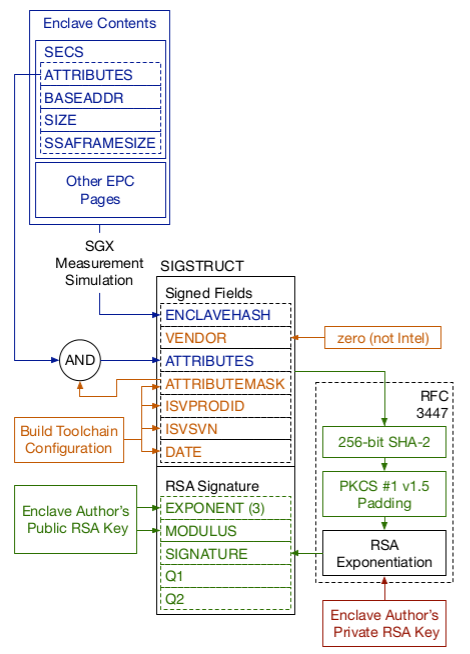
\includegraphics[scale=.3]{img/sgx/enc_id.png}
\caption{Enclave Identity Exchange \protect\cite{Costan_Devadas_2016}}
\end{figure}


\textbf{Enclave Measurement}: A measurement allows a third party to verify what software is running in an enclave for authentication purposes. The third party compares the measurement provided by the enclave to the expected measurement obtained by the remote attestation server (and traced back to Intel provisioning). As described above, an enclave is built using a series of EADD and similar instructions. When publishing an enclave for deployment the author also provides the sequence of instructions that will allow the enclave state to be recreated. This series of instructions is hashed using 256-bit SHA-2 to create its measurement. SHA-2 is a block hash (64byte blocks) that generates a 32byte value. This value is augmented with the enclave specific geometry in MRENCLAVE and the resulting 64byte value is the enclave measure. Enclave attributes are calculated separately and are required for use in attestation. \cite{Costan_Devadas_2016} speculates this decoupling of measures is most likely to allow for a single measured value to represent an enclave while allowing for multiple deployment scenarios based on specific attributes and target architectures. 

Enclave versioning is also supported in SGX. The use case for this event occurs when software components in the enclave need to be updated without involving the original third party attestation source. Since a software update would invalidate the measure, the solution is to migrate an enclave's secret key to the updated enclave through a certificate based enclave identity transfer scheme. Each enclave generates a one level certificate hierarchy using the proprietary SIGSTRUCT format. The information in the certificates supports reasoning about the identity of two related enclaves running different software versions. Included in the SIGSTRUCT are ENCLAVEHASH (the enclaves measurement), ISVPRODID (distinguishes modules signed by a common private key), and other fields used to reason about the enclave's identity. The certificates are signed with RSA using the 256 bit SHA-2 to reduce input size. Currently the SGX implementation only supports 3072-bit RSA keys with a public exponent of 3. This key is used to issue a certificate that identifies the enclaves author. If two enclaves have the same author and software as defined in their attributes, the enclave with the highest security version number (ISVSVN) receives the key. 


\textbf{Software Attestation} - Software attestation is the mechanism used by Intel's attestation server to calculate the measurement of each enclave on a system to remotely verify enclave integrity and establish a secure channel from the quoting enclave (requestor) to the enclave to be verified. Implementation uses ECDH key negotiation between quoting enclave and target enclave to exchange a quote containing the enclave hash, signature from EPID, and security version. This quote is then provided back to the request originator. The attestation key used by the quoting enclave is issued by the Intel controlled Provisioning Enclave after the QE has left the factory. 


The Quoting Enclave used in remote attestation uses an undocumented crypto scheme to verify the enclave's measurement using EREPORT, signs the report as an EPID group member, and creates the quote to be verified by the Intel remote attestation server. Each time a quote is prepared, the QE creates a 16byte key and a 12byte random initialization vector. Random IV ok in this case since the key is always random as well, but in general random IV's are susceptible to attack (see BEAST and other chosen plaintext attacks). Essentially QE process creates a new symmetric key and encrypts it using RSA. It then uses this key with AES-GCM to encrypt the signature with a random IV. The quote produced comes with the encrypted key, a decrypted signature, and a hash of the key. This is an example of hybrid crypto system, combining a private key and public key schemes (AES and RSA see IND-CCA(OAEP) and IND-CPA(GCM)). SHA-256(K) leaks key hash so time-memory tradeoff attacks possible for small keys. RSA doesn't provide forward secrecy. RSA2048 ~ 90bits of security. 


\begin{figure}[H]
\centering
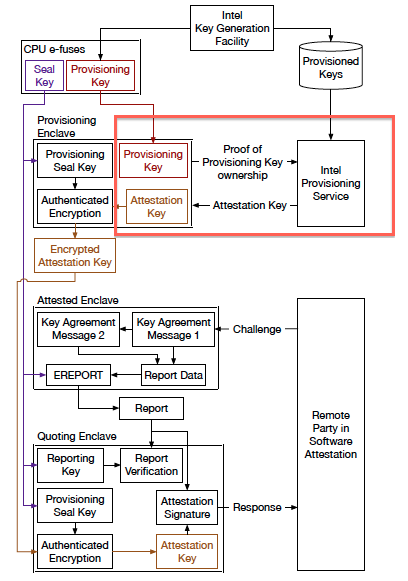
\includegraphics[scale=.5]{img/sgx/sgx_key_attestation.png}
\caption{Remote Key Attestation \protect\cite{Costan_Devadas_2016}}
\end{figure}

The Sealing key encrypts secrets inside the enclave using AES-GCM. The key is derived from the root sealing key and the enclave or signer identity EPID. Sealing provides confidentiality as well as replay protection to the enclave. After provisioning has occurred, the quoting enclave uses EGETKEY to retrieve the seal provisioning key which is used to decrypt the attestation key from the system software. The QE then signs the hash in the attestation report with the attestation key to validate the request.

\textbf{Attack Surface}: Intel acknowledges that SGX won't prevent certain types of attacks. These include cache-timing attacks described below, as well as physical attacks on the chip itself. In general, if the application to be shielded with SGX is insecure, then SGX makes no claim to be able to secure it. 

\textbf{Standard Crypto Algsorithms}: Summary of algorithms identified in use by SGX. Based on IPP 8.2 (Intel's proprietary crypto library) 

* RSA-3072 PKCS 1.5 SHA-256 for enclave signing

* ECDSA over p256 curves, SHA256 for launch enclave policy checks

* ECDH and ECDSA (p256, SHA-256) for remote key exhange

*AES-128 in CTR, GCM, CMAC. GCM for sealing, CMAC for key derivation,

* 128-bit security except for RSA-3072 (~112-bits security)

\textbf{Custom Crypto:}

* Mem encryption engine (HW) see Gueron's RWC'16 talk

** new universal hash-based MAC (provably secure)

** AES-CTR with custom counter block to encrypt inline memory

AES is vulnerable to side-channel attacks. 

\cite{SGXinpractice}


EPID\cite{Brickell_Li_2009}: Enhanced Privacy ID is a group signature scheme where a group of CPUs with the same security version can sign a piece of data, but it's not possible to determine which member of the group signed it. This was developed by Intel to prevent tracking of individual CPUs and is defined in (ISO/IEC 20008-2:2013). EPID uses Baretto-Naehrig EC. Intel's key provisioning service issues the Group Public Key and stores the private Master Issuing Key for use in creating Member Private Keys for provisioning enclaves. 


\begin{figure}[H]
\centering
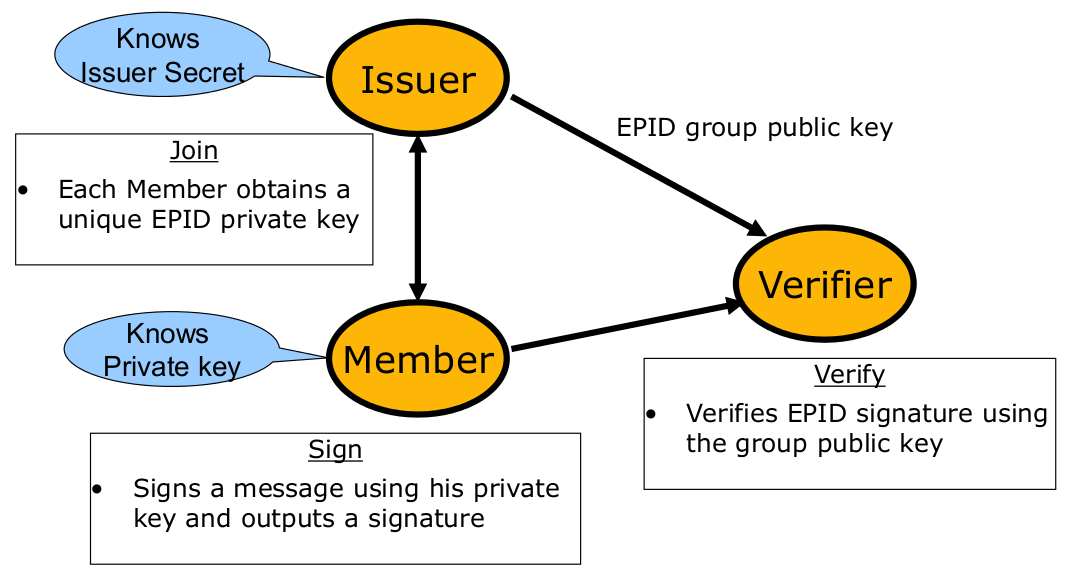
\includegraphics[scale=.2]{img/sgx/epid.png}
\caption{EPID Overview \protect\cite{Brickell_Li_2009}}
\end{figure}





\subsection{Attacking SGX}

\begin{figure}[H]
\centering
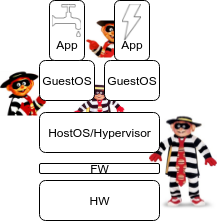
\includegraphics[scale=.7]{img/storm_cellar/threat_model_001.png}
\caption{Threat Model}
\label{fig:threat_model}
\end{figure}


\cite{Schwarz_Weiser_Gruss_Maurice_Mangard_2017} describes an implemented attack which recovers RSA secret keys from an SGX protected enclave. A summary of the attack follows to demonstrate that being relatively new technology, SGX still has some bugs to work out. 

The technique is referred to as a Prime and Probe attack since the attackers use an offline version of the targeted system to determine page access sequences that can uniquely identify the memory blocks used by the target service during the authentication phase. Once the pages have been identified, the attack is 'primed' and the live system is then 'probed' to recover secret keys held in memory during authentication.The threat model assumes the attacker can deploy an enclave on the same system as the victim, and that the victim is using SGX enclaves correctly. It is noted that a side-effect of the protections provided by shielding is that if malicious application enclaves can be deployed, they are invisible to standard system protections such as host based IDS and antivirus. 

% \graphicspath{ {pics/} }
\begin{figure}[H]
\centering
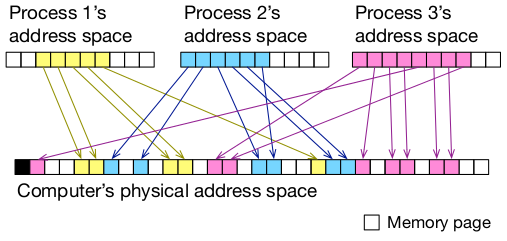
\includegraphics[scale=.4]{img/sgx/paging.png}
\caption{Enclave Paging \cite{Xu_Cui_Peinado_2015}}
\end{figure}
The attacker begins by deploying an enclave running the targeted application, in this case mbedTLS. Since the enclave prevents syscalls a high resolution timer is created from fast running instructions (register add or inc) whose throughput is documented in the SGX specifications.


 Using known similarities between physical and virtual address formats along with the high resolution timer, the researchers demonstrated how it was possible to identify enclave memory cache regions in physical memory using row conflict timings. The result being that the virtual addresses that translate to physical addresses, known as the eviction set, can be identified without triggering the virtual address access protections provided by SGX. 

% \graphicspath{ {pics/} }
\begin{figure}[H]
\centering
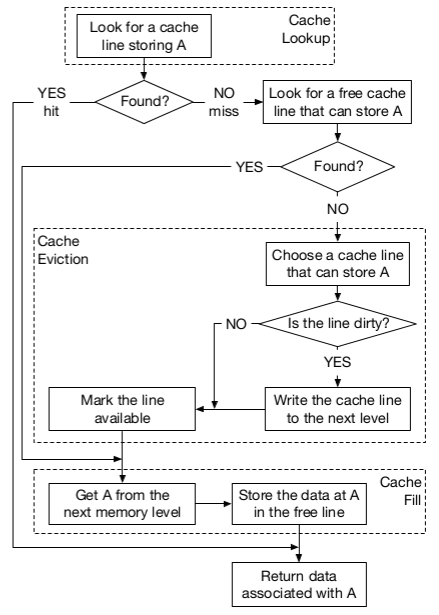
\includegraphics[scale=.5]{img/sgx/cache.png}
\caption{Cache Resolution Process \cite{SGXinpractice}}
\end{figure}

The attacker proceeds to monitor private cache accesses on the controlled enclave running mbedTLS. Timing call traces to the cache during authentication attempts produces a pattern that can be used to isolate the pages involving the client's private key. Through tuning several partial keys are recovered which are then coalesced into the original key. It's interesting to note that larger key sizes actually improve the ability to recover keys as larger key buffers are needed in operation leading to an improved measurement resolution using this technique. It follows that, with the relevant cache access pattern known, the attacker deploys the malicious application enclave to the host where the victim resides and uses the same pattern learned through experimentation to recover the private keys of users authenticating to the victim's enclave. Details on bypassing ASLR and other technical challenges not related to SGX are omitted here for brevity. The results were that full key recovery was accomplished in 11 traces within 5 minutes of the attack start time.\cite{Schwarz_Weiser_Gruss_Maurice_Mangard_2017}

\cite{Xu_Cui_Peinado_2015} uses a page-fault transfer technique to recover and render images being displayed on a victim enclave shielded by SGX. The methodology is similar to \cite{Schwarz_Weiser_Gruss_Maurice_Mangard_2017} in that the target system is emulated in the attacker's test environment. In this case the fingerprint being captured is the unique sequence of page faults the target service generates when the attacker has control of the host fault handling mechanism. Once the sequence is learned the attacker can deploy the malicious enclave adjacent to the victim and with fairly good precision force the page faults at the desired address to exfiltrate the shielded data.The attack takes advantage of misaligned page boundaries to identify the location of the target address space through indirect means.

The 'priming' starts with the target system deployed on an environment the attacker controls under no shielding. The application is run and page fault accesses are traced by preventing access to all pages. The fault address is logged and the application is allowed to resume, resulting in learning the fault addresses at every single byte rather than for a 4Kb page. .

Each fault produces two addresses, the address which triggered the fault and the address of the instruction called. Control transfers sequences are then derived from the fault traces and tuned to the application being targeted. ASLR is accounted for and the attack is then staged on the shielded host. The assumptions made about SGX are that it can still throw page faults on invalid access attempt and that page faults during enclave execution kick over to the operating system fault handler defined in the interrupt descriptor table. 

Given the attacker has control of the host, the attack replaces the default page fault exception handler routine with the one customized in the 'priming' phase. The result being that between 60 and 90 \% of the image data was recoverable across three distinct targets. While not accurate enough for key recovery, the images leaked from memory are easily distinguishable and measures could be taken to improve accuracy if needed. 

% \graphicspath{ {pics/} }
\begin{figure}[H]
\centering
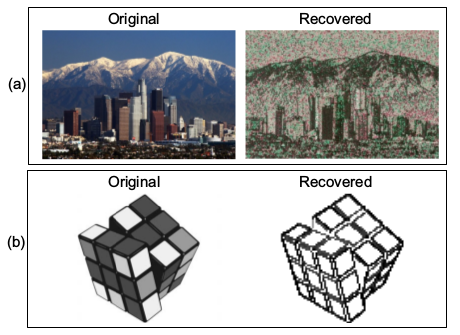
\includegraphics[scale=.5]{img/sgx/img_recov.png}
\caption{Images recovered from \cite{SGXinpractice}}
\end{figure}



% \section{Conlusion}

Intel's SGX provides an additional layer of protection for applications running on untrusted systems. The threat of a compromised hypervisor or operating system gaining control of a less privileged application is largely mitigated through the use of cryptography throughout the enclave lifecycle. If a trusted application can be deployed to an environment that implements SGX it has been shown that any tampering or sniffing an adversary attempts will be severely impeded. 

That said, the cultural changes involved with the development and deployment of applications in secure enclaves could be too high of a hurdle for the majority of businesses to overcome. Whether it is because the inherent security features of SGX prevent standard corporate information assurance processes from being effective, or because the deployment costs to support the application may be more than the value of the data being protected, the return on investment should be considered carefully before adopting SGX. 

The implications of the SGX security paradigm are significant. Understanding of the data and code to be protected is necessary during development, as the enclave Trusted Computing Base (TCB) must be explicitly instructed to secure specific regions of the application software. While the confidentiality and integrity protections may seem appealing at first, it must be considered that existing information assurance applications such as anti virus and intrusion detection systems are prevented from accessing enclave memory regions as well. Hypervisor snapshots containing memory dumps for incident response and forensic investigations are prohibited. Also, debugging or patching a running enclave is prevented, making it difficult for developers to track down issues in production that can't be reliably reproduced in development and testing networks. Adopting SGX would be a major shift from the way many businesses develop applications today.

A popular use case for the technology is in digital rights management. DRM is used to prevent piracy and unauthorized distribution of digital media. It has been a point of contention in both principal and practice for many people. The Sony DRM \cite{Sony_DRM} implementation effectively installed a rootkit on user's computer's that allowed remote attackers to take control of their systems. In theory, an SGX enabled DRM solution would allow vendors to provide software or other digital media to consumers by encrypting it with the customer's identity key and sealing it in a trusted enclave for distribution. The customer would load the product onto the SGX enabled device and proceed with fair use without the ability to copy, modify, or reverse engineer the product since it would be strong encrypted. Further, the vendor would be able to track usage since the product would perform remote attestation every power cycle, and also would be able to revoke the enclave key whenever a license expired or terms of use were violated. 

Obviously this would require wide consumer adoption of SGX (which Intel may be hoping for eventually) but currently the marketing effort is focused on cloud service providers that have an appetite for commodity hardware that will deploy to their data centers and add value to their service offerings. A hurdle for wide scale adoption is with Intel inserting themselves into the attestation chain for all transactions, a position the company could find tenuous if competitors or foreign or domestic governments acting as customers had a bad experience and were feeling punitive. 

While attacks on SGX have been demonstrated, the exploit vectors were complex and in some ways contrived. The SGX architecture was first introduced in the Skylake chipset released in 2015, so we can expect several iterations to pass before rigorous community testing has been done. To that end, early adopters may have a difficult time finding support for enclaves they develop now and may wait for large CSPs to announce investment before pursuing further. It's likely that the SGX will continue to evolve as more security research is conducted and more information is made public. 


% \subsection{Citations}

